\documentclass[12pt,a4paper]{article}
\usepackage[utf8]{inputenc}
\usepackage[T1]{fontenc}
\usepackage[polish]{babel}
\usepackage{amsmath}
\usepackage{amssymb}
\usepackage{graphicx}
\usepackage[a4paper, margin=2.5cm]{geometry}
\usepackage{hyperref}
\usepackage{float}
\usepackage{caption}
\usepackage{booktabs} % Lepsze tabele
\usepackage{xcolor}
\usepackage{longtable} % Dla długich tabel

% Ustawienia dla linków w dokumencie
\hypersetup{
    colorlinks=true,
    linkcolor=blue,
    filecolor=magenta,      
    urlcolor=cyan,
    pdftitle={Sprawozdanie Lista 4: Uczenie Maszynowe},
    pdfauthor={Bartosz Gotowski}
}

\newcommand{\code}[1]{\texttt{\detokenize{#1}}}

\title{\LARGE \textbf{Sztuczna inteligencja i inżynieria wiedzy}\\[0.5em]
\large Lista 4: Uczenie Maszynowe — Klasyfikacja}
\author{Bartosz Gotowski}
\date{11 czerwca 2025}

\begin{document}

\maketitle
\begin{center}
    \textit{Sprawozdanie z realizacji projektu dotyczącego klasyfikacji wzorców morfologicznych płodu na podstawie danych z kardiotokogramu (CTG).}
\end{center}
\vspace{1cm}

\tableofcontents
\clearpage

\section{Wprowadzenie}
Celem niniejszego ćwiczenia było praktyczne zastosowanie algorytmów uczenia maszynowego do rozwiązania problemu klasyfikacji wieloklasowej. Monitorowanie stanu zdrowia płodu za pomocą kardiotokografii (CTG) jest kluczowym elementem opieki prenatalnej. Automatyzacja analizy zapisów CTG ma potencjał do wspierania personelu medycznego w podejmowaniu szybkich i trafnych decyzji diagnostycznych, co bezpośrednio wpływa na bezpieczeństwo matki i dziecka.

Zadanie polegało na identyfikacji typu wzorca morfologicznego płodu (1 z 10 klas) na podstawie 21 cech diagnostycznych. Projekt obejmował pełen cykl życia modelu uczenia maszynowego, począwszy od eksploracji danych, przez ich przygotowanie i modelowanie, aż po ewaluację i wyciągnięcie wniosków.

W sprawozdaniu przedstawiono następujące etapy:
\begin{enumerate}
    \item \textbf{Eksploracja danych:} Analiza statystyczna i wizualna zbioru w celu zrozumienia jego charakterystyki.
    \item \textbf{Przygotowanie danych:} Opracowanie strategii radzenia sobie z brakującymi wartościami oraz testowanie metod przetwarzania danych, takich jak standaryzacja i redukcja wymiarowości (PCA).
    \item \textbf{Klasyfikacja:} Zastosowanie i porównanie algorytmów: Naiwnego Klasyfikatora Bayesa, Drzewa Decyzyjnego, Lasu Losowego i Maszyny Wektorów Nośnych (SVM).
    \item \textbf{Ocena i Wnioski:} Analiza wyników przy użyciu odpowiednich metryk i wyciągnięcie wniosków końcowych.
    \item \textbf{Analiza Bonusowa:} Zbadanie techniki przycinania drzewa decyzyjnego jako metody walki z przeuczeniem.
\end{enumerate}

\section{Eksploracja Danych}
\subsection{Struktura i Właściwości Zbioru}
Zbiór danych składa się z 2126 próbek i 22 kolumn. Każda z 21 cech jest typu numerycznego, a kolumna \code{CLASS} reprezentuje etykietę docelową. Kluczowym zaobserwowanym problemem była obecność brakujących wartości w każdej kolumnie cech (od 85 do 132 braków), co wymusiło zastosowanie strategii ich uzupełniania (imputacji).

\subsection{Rozkład Klas}
Analiza rozkładu klas (Rysunek \ref{fig:class_dist}) wykazała, że zbiór danych jest \textbf{silnie niezbalansowany}. Klasa \code{2} jest najliczniejsza (ponad 550 próbek), podczas gdy najrzadsza klasa \code{3} ma ich tylko 53. Ta nierównowaga jest krytyczna dla procesu modelowania i oceny – klasyfikator mógłby osiągnąć wysoką dokładność, faworyzując najczęstsze klasy. Z tego powodu do oceny modeli wykorzystano metryki odporne na ten problem, jak ważony F1-score.

\begin{figure}[H]
    \centering
    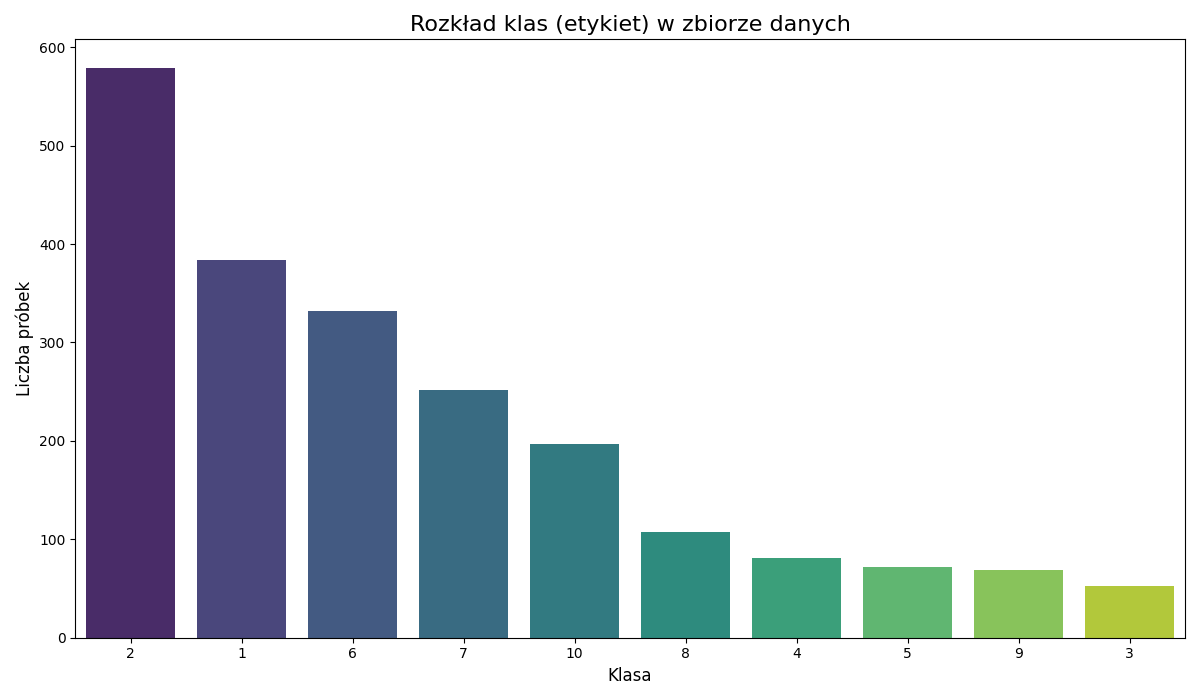
\includegraphics[width=0.8\textwidth]{output/class_distribution.png}
    \caption{Niezbalansowany rozkład 10 klas wzorców morfologicznych w zbiorze danych.}
    \label{fig:class_dist}
\end{figure}

\subsection{Rozkład Cech}
Wizualizacja histogramów dla poszczególnych cech (Rysunek \ref{fig:feature_hist}) ujawniła zróżnicowaną naturę danych. Cechy takie jak \code{LB} (bazowe tętno płodu) czy \code{Mode} mają rozkłady zbliżone do normalnego. Z kolei wiele cech, np. \code{FM} (ruchy płodu) czy \code{DS} (poważne spowolnienia), jest silnie prawostronnie skośnych, co jest zjawiskiem oczekiwanym, gdyż reprezentują one zdarzenia rzadkie, ale klinicznie istotne. Duża rozpiętość skali wartości między cechami (np. \code{AC} vs \code{Width}) sugeruje, że algorytmy wrażliwe na odległość (jak SVM) odniosą korzyść ze standaryzacji.

\begin{figure}[H]
    \centering
    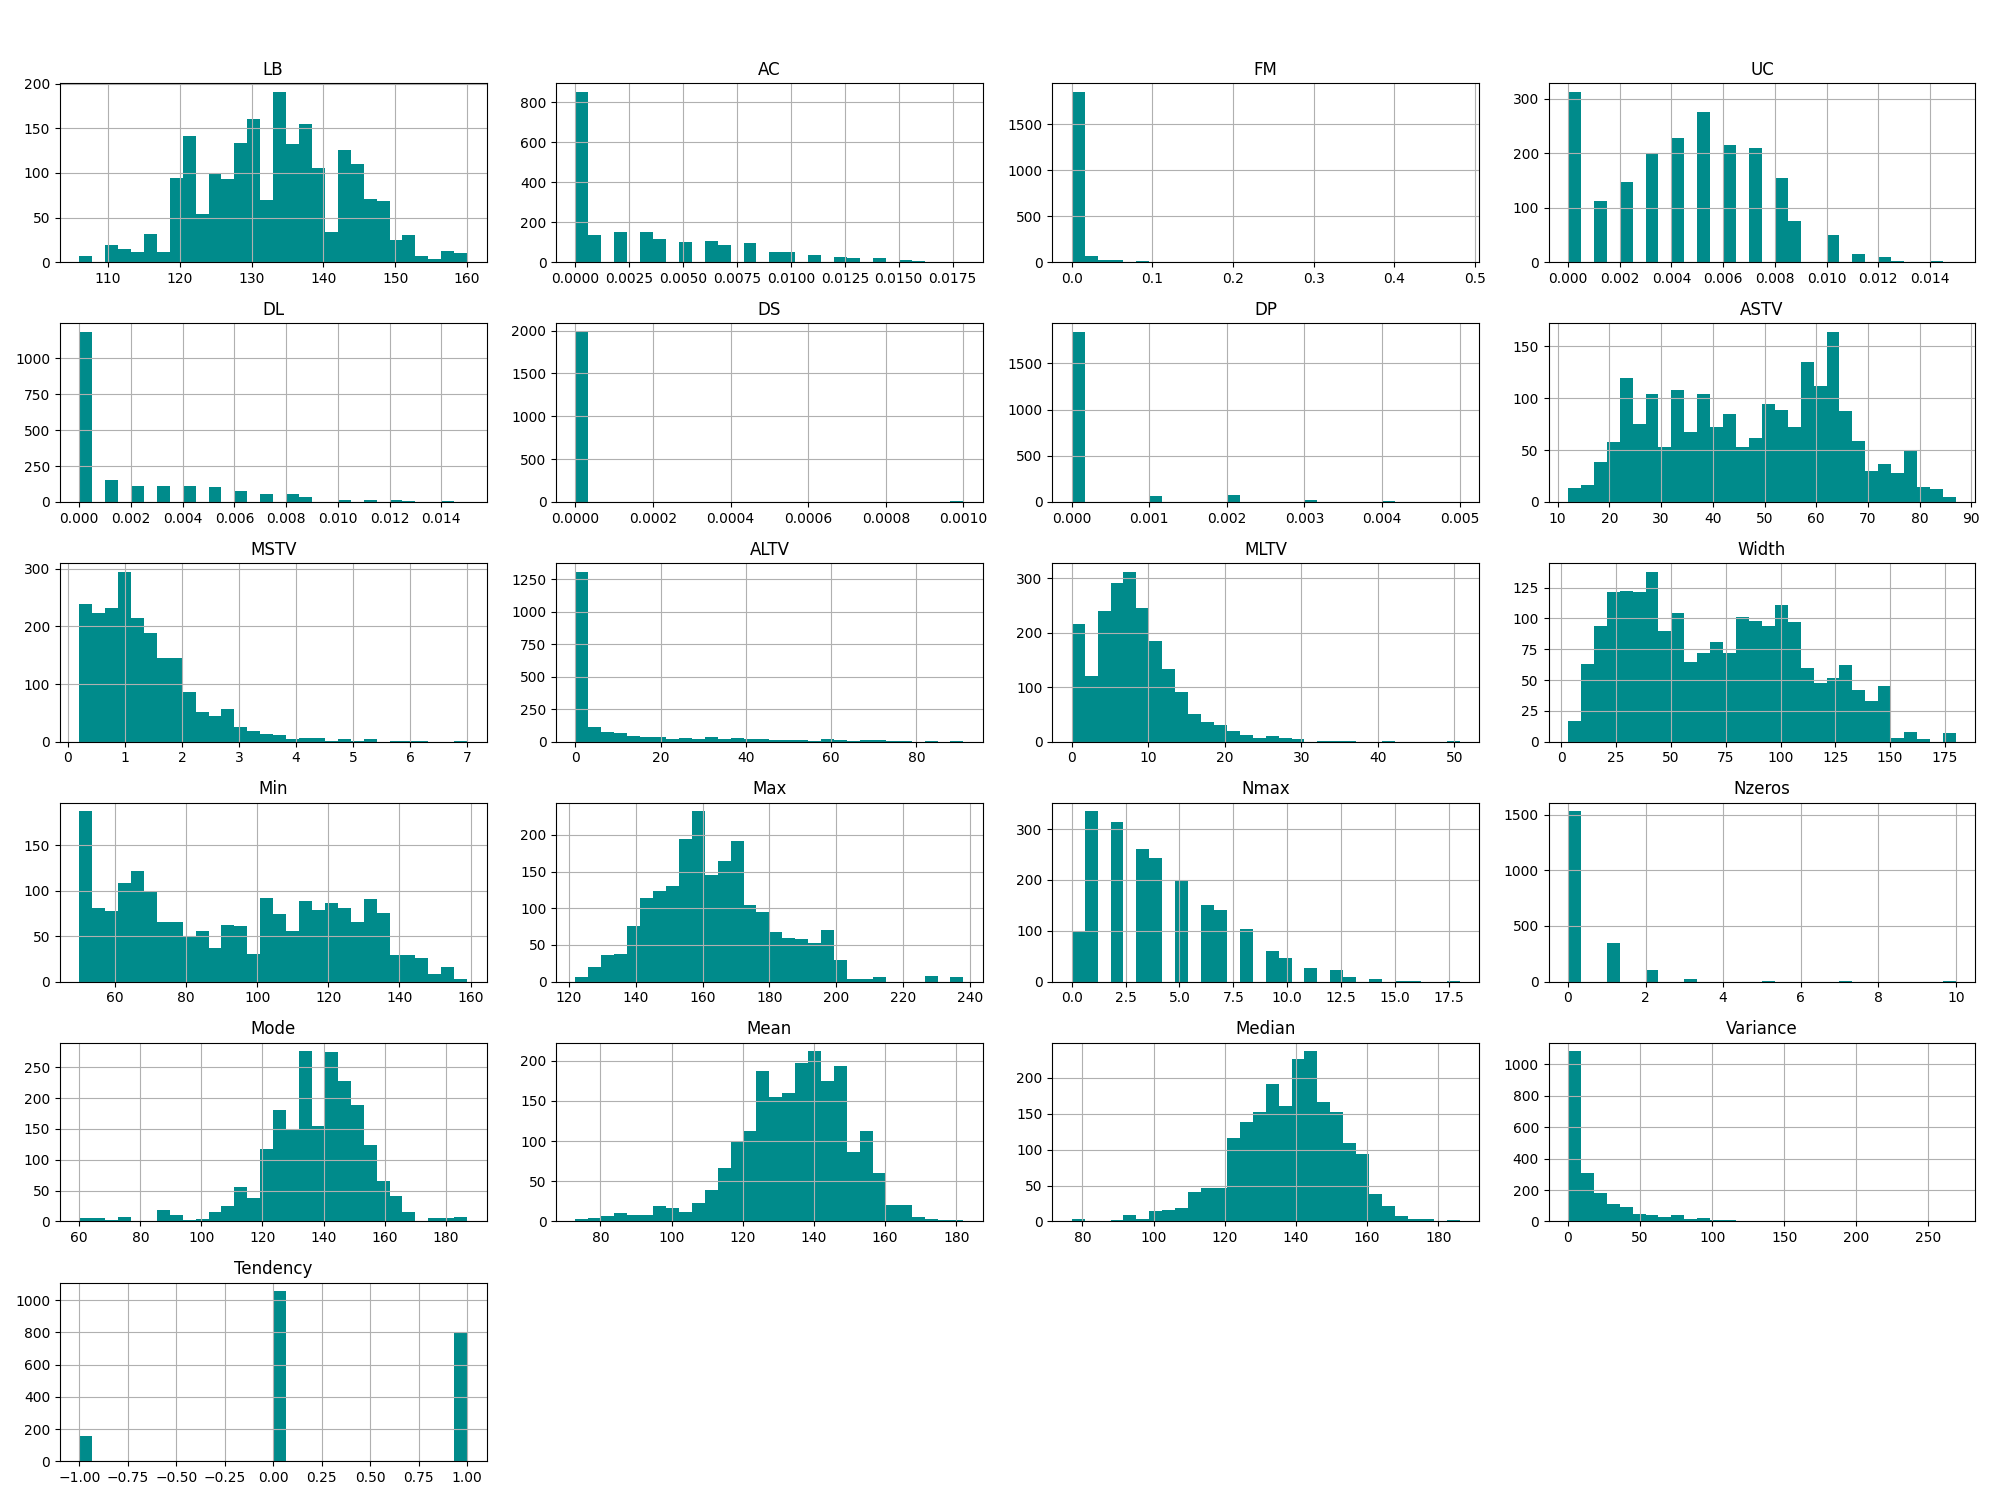
\includegraphics[width=\textwidth]{output/feature_histograms.png}
    \caption{Histogramy rozkładów wartości dla cech diagnostycznych.}
    \label{fig:feature_hist}
\end{figure}

\clearpage

\section{Przygotowanie Danych i Metodyka Eksperymentu}
W celu zapewnienia rzetelności i powtarzalności, zastosowano ustrukturyzowane podejście oparte na potokach (\code{Pipelines}) z biblioteki \code{scikit-learn}.
\subsection{Podział Danych}
Zbiór danych został podzielony na zbiór uczący (80\%) i testowy (20\%). Zastosowano \textbf{stratyfikację} względem kolumny \code{CLASS}, aby zapewnić, że proporcje klas w obu podzbiorach są identyczne jak w całym zbiorze.

\subsection{Potoki Przetwarzania Danych}
Zdefiniowano trzy strategie przygotowania danych, zaimplementowane jako osobne potoki:
\begin{enumerate}
    \item \textbf{Brak przetwarzania:} Uzupełnienie brakujących wartości medianą.
    \item \textbf{Standaryzacja:} Imputacja medianą, a następnie skalowanie cech za pomocą \code{StandardScaler}.
    \item \textbf{PCA:} Imputacja, standaryzacja i redukcja wymiarowości przez PCA z zachowaniem 95\% wariancji.
\end{enumerate}

\subsection{Walidacja Krzyżowa}
Do oceny modeli na zbiorze uczącym wykorzystano \textbf{5-krotną stratyfikowaną walidację krzyżową}, co pozwoliło uzyskać stabilną i wiarygodną ocenę wydajności każdego modelu.

\section{Wyniki Klasyfikacji i Ocena}
\subsection{Porównanie Modeli w Walidacji Krzyżowej}
Tabela \ref{tab:cv_results} przedstawia uśrednione wyniki F1-score uzyskane w procesie walidacji krzyżowej.

\begin{table}[H]
    \centering
    \caption{Wyniki 5-krotnej walidacji krzyżowej (posortowane wg F1-score).}
    \label{tab:cv_results}
    \small
    \begin{tabular}{llcc}
        \toprule
        \textbf{Przetwarzanie} & \textbf{Klasyfikator} & \textbf{Średni F1-score} & \textbf{Odch. std. F1} \\
        \midrule
        Brak przetwarzania & Las Losowy (Bonus) & 0.841 & 0.014 \\
        Standaryzacja & Las Losowy (Bonus) & 0.840 & 0.018 \\
        Brak przetwarzania & Drzewo (min\_leaf=5) & 0.767 & 0.025 \\
        Brak przetwarzania & Drzewo (domyślne) & 0.766 & 0.019 \\
        Standaryzacja & Drzewo (domyślne) & 0.765 & 0.020 \\
        Standaryzacja & Drzewo (min\_leaf=5) & 0.765 & 0.025 \\
        Standaryzacja & SVM (Bonus) & 0.763 & 0.025 \\
        PCA (95\% wariancji) & SVM (Bonus) & 0.742 & 0.016 \\
        PCA (95\% wariancji) & Las Losowy (Bonus) & 0.735 & 0.019 \\
        Brak przetwarzania & Drzewo (max\_depth=5) & 0.726 & 0.021 \\
        Standaryzacja & Drzewo (max\_depth=5) & 0.726 & 0.020 \\
        PCA (95\% wariancji) & Drzewo (min\_leaf=5) & 0.615 & 0.021 \\
        PCA (95\% wariancji) & Drzewo (domyślne) & 0.611 & 0.018 \\
        PCA (95\% wariancji) & Naiwny Bayes & 0.604 & 0.035 \\
        Standaryzacja & Naiwny Bayes & 0.603 & 0.017 \\
        Brak przetwarzania & Naiwny Bayes & 0.553 & 0.032 \\
        PCA (95\% wariancji) & Drzewo (max\_depth=5) & 0.526 & 0.017 \\
        Brak przetwarzania & SVM (Bonus) & 0.470 & 0.015 \\
        \bottomrule
    \end{tabular}
\end{table}

Wyniki jednoznacznie wskazują, że metody zespołowe (Las Losowy) znacznie przewyższają pojedyncze klasyfikatory.

\subsection{Ocena Końcowa Najlepszego Modelu}
Na podstawie wyników walidacji, jako finalny model wybrano Las Losowy z podstawowym potokiem przetwarzania. Model został wytrenowany na całym zbiorze uczącym i oceniony na zbiorze testowym (Tabela \ref{tab:final_report}, Rysunek \ref{fig:final_cm}).

\begin{table}[H]
    \centering
    \caption{Raport klasyfikacji dla Lasu Losowego na zbiorze testowym.}
    \label{tab:final_report}
    \small
    \begin{tabular}{lrrrr}
        \toprule
        \textbf{Klasa} & \textbf{Precyzja} & \textbf{Czułość} & \textbf{F1-score} & \textbf{Liczba próbek} \\
        \midrule
        1 & 0.84 & 0.87 & 0.85 & 77 \\
        2 & 0.83 & 0.93 & 0.88 & 116 \\
        3 & 0.75 & 0.27 & 0.40 & 11 \\
        4 & 0.70 & 0.44 & 0.54 & 16 \\
        5 & 0.80 & 0.29 & 0.42 & 14 \\
        6 & 0.88 & 0.85 & 0.86 & 67 \\
        7 & 0.88 & 0.82 & 0.85 & 51 \\
        8 & 0.91 & 0.95 & 0.93 & 21 \\
        9 & 0.93 & 1.00 & 0.97 & 14 \\
        10 & 0.81 & 0.97 & 0.88 & 39 \\
        \midrule
        \textbf{Dokładność} & & & \textbf{0.85} & \textbf{426} \\
        \textbf{Średnia ważona} & \textbf{0.84} & \textbf{0.85} & \textbf{0.83} & \textbf{426} \\
        \bottomrule
    \end{tabular}
\end{table}
\begin{figure}[H]
    \centering
    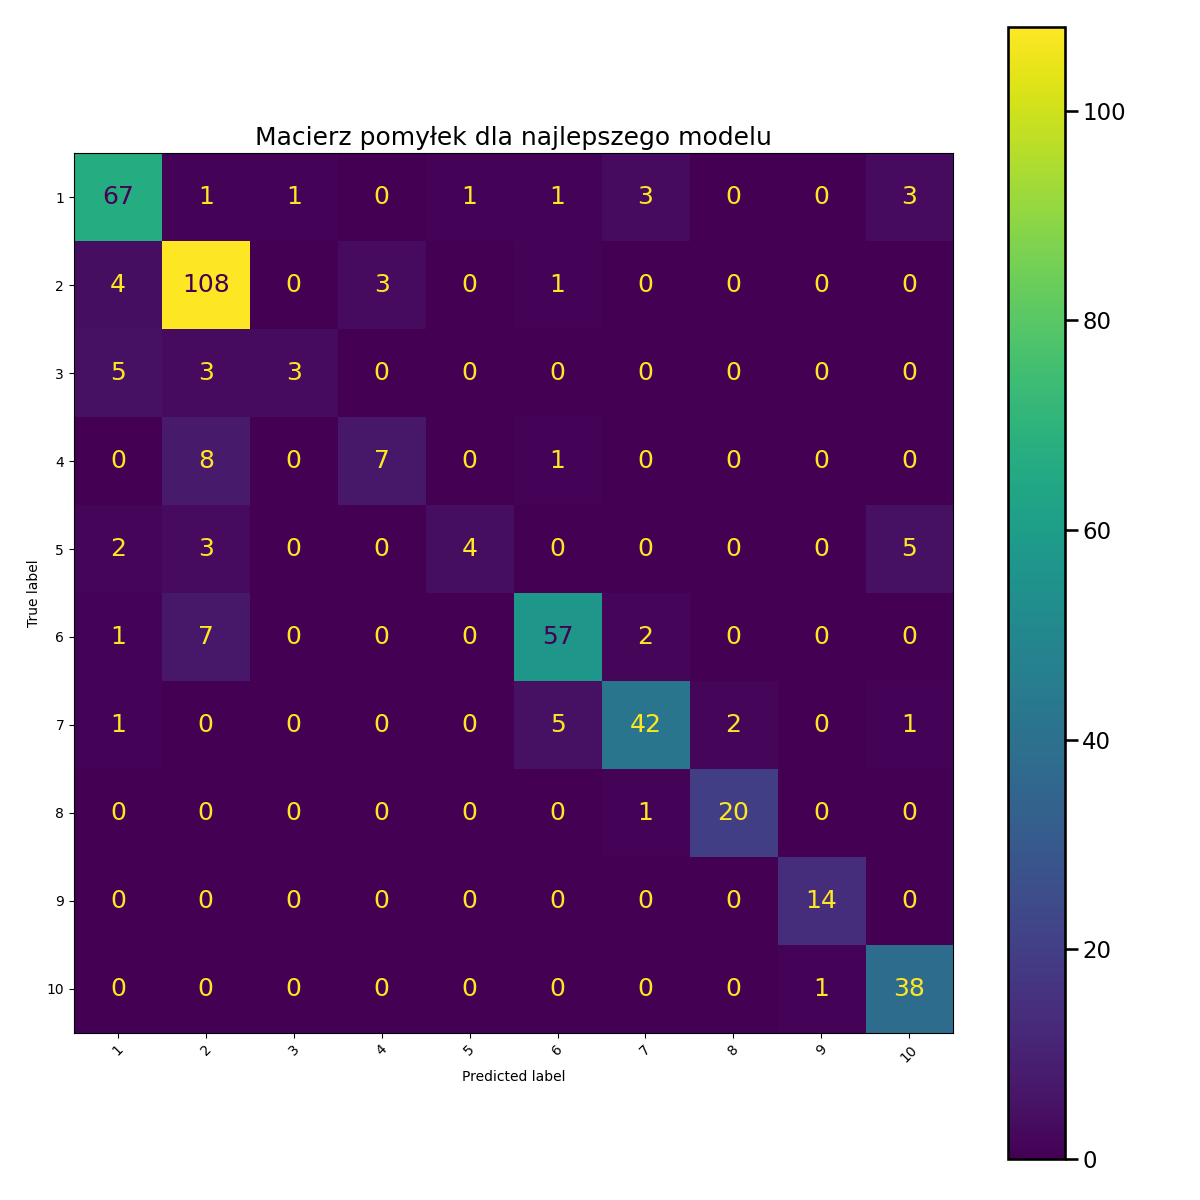
\includegraphics[width=0.7\textwidth]{output/best_model_confusion_matrix.png}
    \caption{Macierz pomyłek dla Lasu Losowego na zbiorze testowym.}
    \label{fig:final_cm}
\end{figure}
Model uzyskał F1-score na poziomie 0.83, co potwierdza jego dobrą generalizację. Macierz pomyłek pokazuje, że największym wyzwaniem jest niska czułość dla klas mniejszościowych (np. 3 i 5). Może to sugerować, że cechy diagnostyczne dla tych wzorców są do siebie podobne, lub że model, z powodu małej liczby przykładów, ma tendencję do wybierania częstszych klas o zbliżonym profilu.

\clearpage

\section{Analiza Bonusowa: Łagodzenie Przeuczenia}
W ramach zadania dodatkowego zbadano wpływ techniki \textbf{Cost-Complexity Pruning} na Drzewo Decyzyjne. Technika ta ilustruje kompromis między wariancją a obciążeniem modelu.
\begin{itemize}
    \item \textbf{Model Domyślny (nieprzycięty):} F1-score (ważony) 0.76, 180 liści, głębokość 21.
    \item \textbf{Model Przycięty ($\text{ccp\_alpha}=0.0016$):} F1-score (ważony) 0.77, 67 liści, głębokość 12.
\end{itemize}
Zastosowanie przycinania \textbf{poprawiło wynik F1-score}, jednocześnie drastycznie \textbf{redukując złożoność modelu} (o 63\% mniej liści). Oznacza to, że model przycięty jest znacznie prostszy, bardziej odporny na przeuczenie i łatwiejszy do interpretacji, nie tracąc przy tym, a nawet zyskując, na jakości predykcji.

\section{Podsumowanie i Wnioski Końcowe}
\begin{enumerate}
    \item \textbf{Las Losowy} okazał się najskuteczniejszym klasyfikatorem dla tego zbioru danych. Jego wysoka wydajność, nawet bez zaawansowanego przetwarzania danych, czyni go modelem z wyboru.
    \item \textbf{Niezbalansowanie klas} jest głównym czynnikiem ograniczającym wydajność modelu, zwłaszcza dla rzadkich wzorców. Dalsze prace powinny skupić się na technikach radzenia sobie z tym problemem, takich jak nadpróbkowanie (np. SMOTE) lub ważenie klas.
    \item \textbf{Przygotowanie danych} ma kluczowe znaczenie. Standaryzacja jest niezbędna dla algorytmów wrażliwych na skalę (SVM), podczas gdy redukcja wymiarowości przez PCA okazała się w tym przypadku niekorzystna.
    \item \textbf{Regularyzacja} (np. przycinanie drzew) jest potężnym narzędziem do tworzenia prostszych, lepiej generalizujących modeli. W przypadku drzewa decyzyjnego, udało się znacząco zredukować jego złożoność przy jednoczesnej poprawie wyników.
\end{enumerate}
W kontekście wdrożenia, rekomendowanym rozwiązaniem byłby model Lasu Losowego. Jeśli jednak priorytetem byłaby pełna interpretowalność decyzji, zoptymalizowane, przycięte Drzewo Decyzyjne stanowiłoby doskonałą alternatywę.

\section*{Materiały Źródłowe}
\begin{enumerate}
    \item Dokumentacja biblioteki \code{scikit-learn}: \href{https://scikit-learn.org/stable/documentation.html}{https://scikit-learn.org/stable/documentation.html}.
\end{enumerate}

\end{document}